% !TeX encoding = windows-1250
% preamble for the RiTeh thesis template

\documentclass[botnum,a4paper,11,oneside,final]{tex_aux/rithesis}
%\usepackage[latin1]{inputenc}
%\usepackage[T1]{fontenc}
%\usepackage[english]{babel}
%%%%%%% adjustment for croatian
\usepackage[croatian]{babel}
\usepackage[cp1250]{inputenc}	% this ensures croatian special letters are correctly printed with Windows
%\usepackage[utf8]{inputenc}		% allegedly this will produc Croatian special letter correctly in Linux
%::::::::::::::::::::::::::::::::::::::::::::::::::::::::::::::::::::::::::::
\usepackage{comment} %za komentiranje \begin{comment}content...\end{comment}
\usepackage{enumitem}  % za reguliranje vertikalnoga razmaka izmedju stavki u listi
%\setlist{noitemsep} % or \setlist{nolistsep} to cancel all separations
\setlist[itemize]{itemsep=0pt, topsep=4pt, partopsep=0pt, parsep=1ex}
\setlist[enumerate]{itemsep=0pt, topsep=4pt, partopsep=0pt, parsep=1ex}
\setlist[description]{itemsep=0pt, topsep=4pt, partopsep=0pt, parsep=1ex}
%\setlist[enumerate,1]{leftmargin=1cm}
%\setlist[enumerate,2]{leftmargin=1.5cm}
%::::::::::::::::::::::::::::::::::::::::::::::::::::::::::::::::::::::::::::
\usepackage{datetime}  % automatic months, years, days
%\newcommand{\MONTH}{% daje error, zamijenjena sa renew:
\renewcommand{\MONTH}{% renew
  \ifcase\the\month
  \or sije�anj% 1
  \or velja�a% 2
  \or o�ujak% 3
  \or travanj% 4
  \or svibanj% 5
  \or lipanj% 6
  \or srpanj% 7
  \or kolovoz% 8
  \or rujan% 9
  \or listopad% 10
  \or studeni% 11
  \or prosinac% 12
  \fi}
%%::::::::::::::::::::::::::::::::::::::::::::::::::::::::::::::::::::::::::::
%\usepackage{setspace}
%\usepackage{lipsum,lineno}
\usepackage[pangram]{blindtext}
\usepackage{ragged2e}   % poravnavanje teksta
\usepackage{graphicx}	% this enables import of graphics
\usepackage[labelsep=space,format=hang]{caption}  % adjusts caption style
\usepackage{subfig}	% this enables use of subfigures
\usepackage{amsmath}
\usepackage{amssymb}
%\usepackage{fancyhdr}
\usepackage{amsfonts}
%\usepackage{amsthm}
%\usepackage{pdfsync}
% This package is used to tell TeXShop where things are in the PDF file.
% Command-click at any spot in the PDF and it will jump to the corresponding
% location in the source file.
\usepackage{epsfig}		% to use eps figures; maybe not necessary to use here with Mac
\usepackage{epstopdf}	% this automatically converts any eps-figure into a pdf-figure
\usepackage[section]{placeins} % da slika ne upada u sljedeci section

\hyphenation{sko-ko-vi-toj}

\DeclareGraphicsRule{.tif}{png}{.png}{`convert #1 `dirname #1`/`basename #1 .tif`.png}	% this converts any tif-figure into a png-figure (Mac directly supports pdf, jpg, png, and mps formats, but additionally can use tif and eps when they are automatically converted in png, and pdf, respectively, using the above two packages
\DeclareGraphicsExtensions{.pdf,.jpeg,.jpg,.png}  % ekstenzije koje ne treba pisati uz ime slike
\graphicspath{{slike/}}   % mjesto gdje su smjestene slike

%\usepackage{makeidx}	% this enables creation of index
%\usepackage{showidx}
%\makeindex			% this makes index automatically, based on author's entries

%\usepackage{eufrak}
%\usepackage[mathcal]{euscript}
\usepackage{psfrag}
%\usepackage{url} 
\usepackage{pdfcomment}
\usepackage{hyperref}
\hypersetup{
breaklinks,
colorlinks=true,
linkcolor=black,
citecolor=black,
filecolor=black,
urlcolor=black
}

\setcounter{topnumber}{1} \setcounter{bottomnumber}{1}

\newcommand{\navod}[1]{``#1''}

\usepackage{glossaries}
\setacronymstyle{long-short}
\makeglossaries

\usepackage{amsthm}
\theoremstyle{definition}
\newtheorem{definition}{Definicija}[section]
%\begin{definition}{pojam} je to i to.\end{definition}
%\definition Pojam je to i to

\usepackage{todonotes} % \todo[inline]{Todo}
\usepackage{cancel} % prekrizeni tekst \cancel{expression}
\usepackage{ulem}
\usepackage{upgreek} % grcki alabet
\usepackage{amssymb} % matematicki simboli
\usepackage{float} % forsira pozicioniranje slike (u odnos na tekst) tamo gdje je komanda \begin{figure}[H] \end{figure}
%\usepackage[numbers]{natbib} % citiranje 2 autora za redom u formatu [3,5] \cite{bibtexkey3,bibtexkey5}
%\usepackage{notoccite}
\usepackage{makecell} % linebreak u celiji tablice:  & \makecell{Prvi red pa\\drugi red u celiji}
\usepackage[table]{colortbl} % oboji celiju tablice &{\cellcolor{green!<tekst celije>}}
\usepackage{pdfpages} % za umetnuti skenirani zadatak (za vlastiti primjerak rada) ili pdf prilog umjeto :\begin{assignmentpage} \end{assignmentpage} staviti: 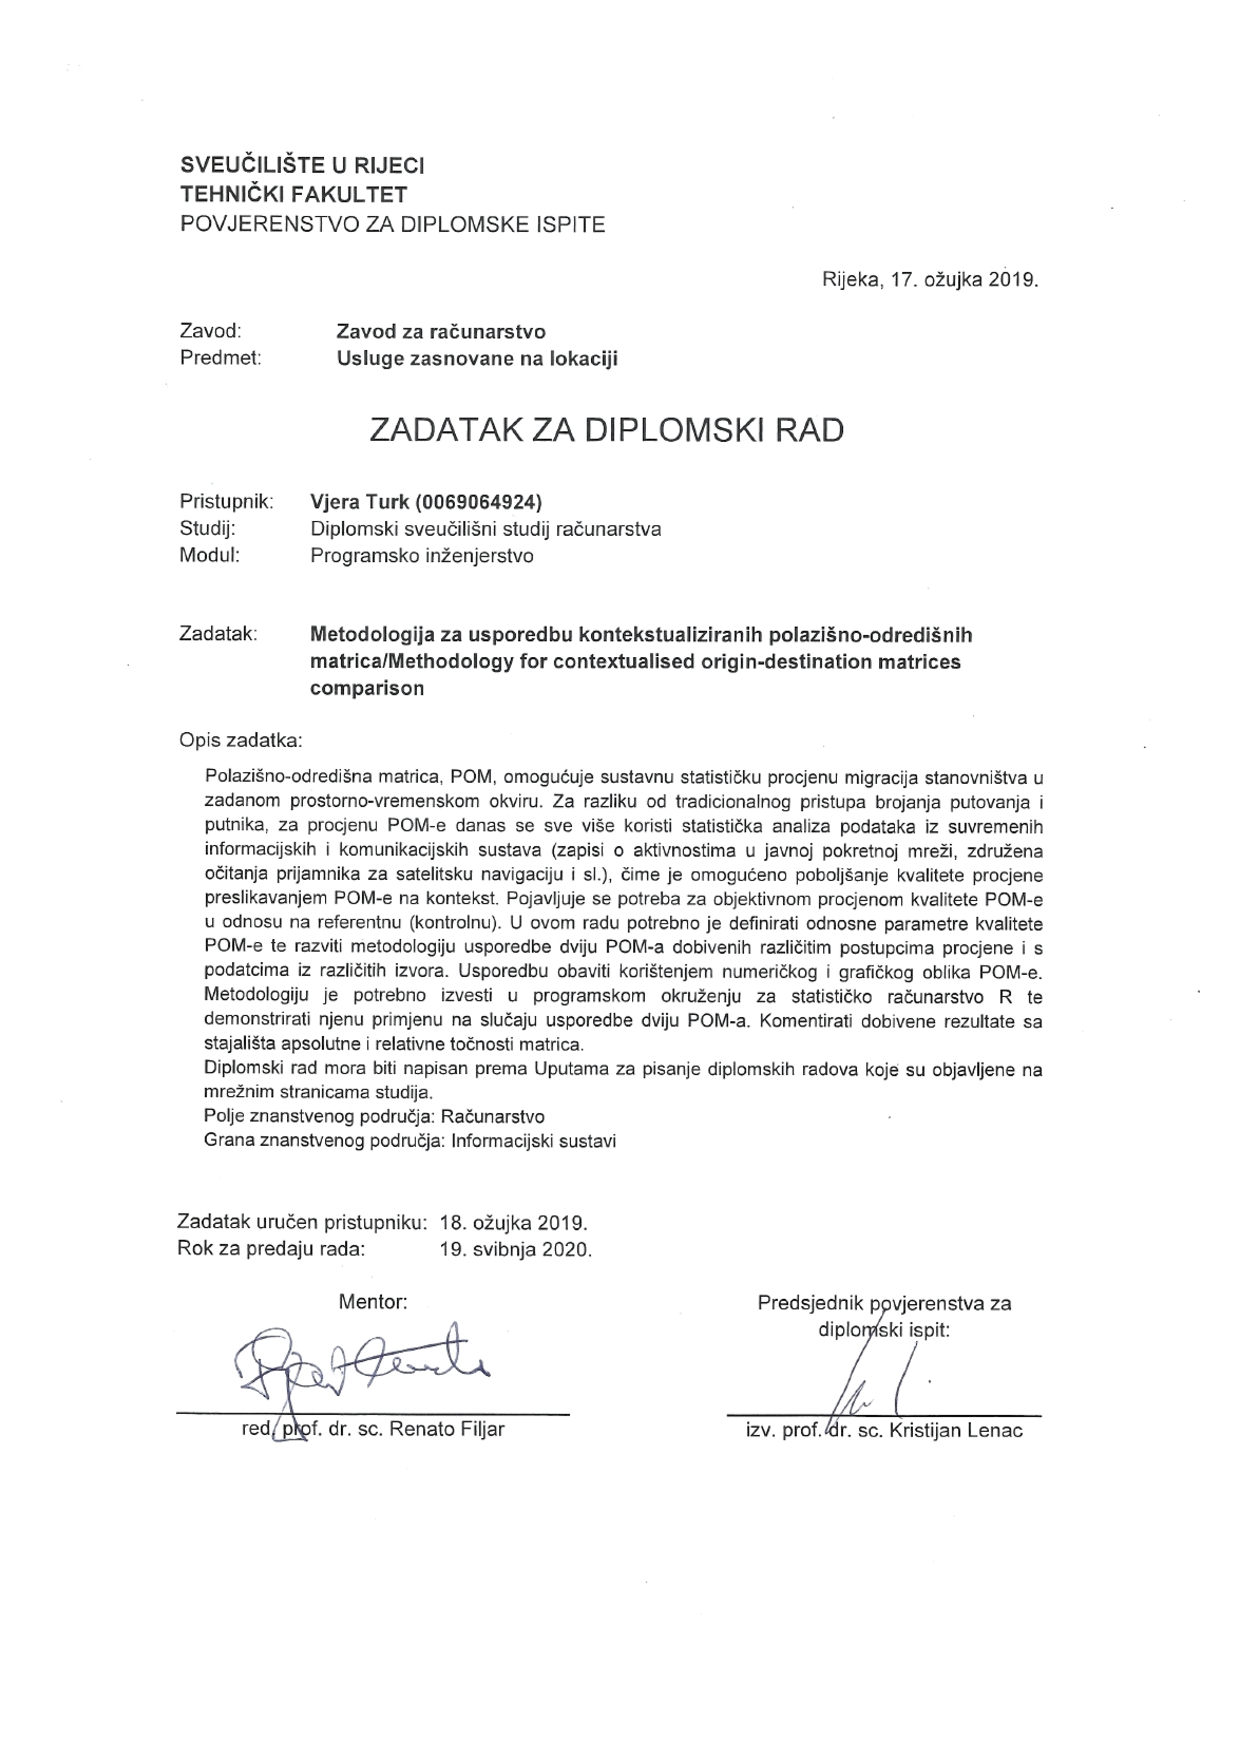
\includepdf[pages=-]{zadatak.pdf}
%\usepackage{subfig}
%\usepackage{floatrow}
\setcounter{tocdepth}{3} % numerira 3. razinu sekcija (4.2.1.1) - (tipicno se koriste samo poglavlje i 2 razine sekcija)
\setcounter{secnumdepth}{3} % dodaje 3. razinu sekcija u Sadrzaj